\documentclass[12pt]{article}   % Précise le type de document, et la taille de la police de caractère
% packages
%----------------------------------------------------------------
% Packages
%----------------------------------------------------------------

\usepackage{natbib} % Pour pouvoir utiliser une bibliographie externe
\usepackage[french]{babel}	% Pour préciser la langue du document
\usepackage[utf8]{inputenc}	% Précise comment le texte est saisi : cela permet de tapper directement les accents
\usepackage[T1]{fontenc}	% Précise la façon dont le document actuel est encodé
\usepackage{setspace}
\usepackage[margin=2.5cm]{geometry} % Précise les marges du document

% Boxes quotation
\usepackage{tcolorbox}

% icones
\usepackage{fontawesome5}

%Sections
%----------------------------------------------------------------
%\usepackage{newclude} % Pour pouvoir utiliser l'étoile après \inculde pour éviter les sauts de page. Ce package a des problême de compatibilité avec la package natbib
%\renewcommand\thesection{} % Pour éviter la numérotation des sections
%----------------------------------------------------------------

%Autres packages et commandes utiles
%----------------------------------------------------------------
\usepackage{amsmath,amsthm,amssymb,amsfonts}	% Pour pouvoir inclure certains symboles et environnements mathématiques
\usepackage{enumerate} % Pour mieux gérer la commande enumerate dans les sections
\usepackage{graphicx}	% Pour inclure des images
\graphicspath{{assets/}}
\usepackage{color}	% Pour inclure du texte en couleur
\usepackage{units}	% Pour pouvoir tapper les unités correctement
\usepackage{pgf,tikz}	% Utilisation du module tikz, qui permet de tracer des belles images
% \usetikzlibrary{arrows} % Quand on exporte une image GeoGebra, on a besoin de préciser cela
\usepackage{hyperref}	% Pour include des liens dans le document
% \usepackage{cprotect}	% Pour pouvoir personaliser la légende des figures
%----------------------------------------------------------------


% variables
\title{Dossier de projet}% N'affecte pas la page titre, mais défini le nom de votre projet
\author{Sofiane MSATFA} % N'affecte pas la page titre, mais défini le nom de l'auteur(e) du projet

%Informations destinées à la page de présentation
%----------------------------------------------------------------
\newcommand{\titre}{Dossier de projet professionnel}
\newcommand{\formation}{Titre professionnel développeur web\\ et web mobile (DWWM)}
\newcommand{\auteur}{Sofiane MSATFA}
\newcommand{\session}{2021-2022}
%----------------------------------------------------------------

% boxe commentaires
\newtcolorbox{commentaire}{
    before=\vspace{0.5cm},
    after=\vspace{0.5cm},
    colframe=blue!40!white,
    colback=blue!8!white
    }

\newcommand{\colored}[1]{{\color{red!55!orange}#1}}

\begin{document}

% page de couverture
\thispagestyle{empty}	% Pour éviter d'avoir un en-tête et un pied de page sur la page couverture


\includegraphics[width=8cm]{logo.jpg}	% Pour inclure le logo (on précise la largeur de l'image)

\vspace{4cm}	% Espacement vertical

\begin{center}	% On centre le texte
    {\huge \bf \titre}\\	% \huge fait que le texte est gros, \bf fait que le texte est gras
    \vspace{4cm}
    {\large \formation}\\
    \vspace{4cm}
    réalisé par \\ \auteur \\
    \vfill	% On va jusqu'au bas de la page avant de mettre le texte ci-dessous
    \session
    \pagebreak
\end{center}
    % Inclut le code contenu dans un fichier comme s'il était entré ici

% table des matières
\tableofcontents

% sections
% Le package newclude mis en commentaire permet d'introduire une * pour éviter le saut de page entre les section
\section{Introduction}

Dans le cadre de ma formation développeur web et web mobile, j’ai eu la chance d’assister Mr. Vincent VAURETTE qui est en charge de la cellule de transition numérique de la Fédération Française de Volley-Ball (FFVB).\\
Le but de son travail est de développer des outils qui facilitent la gestion de tout ce qui est en lien avec le monde du volley-ball, et de redonner un coup de jeune à l’intranet de la fédération.\\
Durant trois mois, j’ai eu la responsabilité de la transition numérique de l’interface de désignation des arbitres.

\vspace{1cm}


\includegraphics{logo.jpg}

La Fédération Française de Volley-Ball est une association créée en 1936 qui constitue l’instance dirigeante du volley-ball en France. 
Plusieurs centaines de matchs se déroulent par week-end, et la désignation des arbitres les concernant est entrêmement chronophage.


\begin{commentaire}
    Le site actuel de la fédération date de 2009 et manque d’ergonomie. Celui-ci demande plusieurs click pour effectuer une seule désignation et ne permet pas d’afficher toutes les informations nécessaires pour celles-ci. Les gestionnaires sont alors contraints de passer par un tableur externe pour procéder aux désignations, puis ensuite de rentrer manuellement celles-ci pour chaque match.
\end{commentaire}


L’objectif principal qui m’a été confié a été la création d’un outil permettant d’automatiser ces désignations. Celui-ci devait pouvoir associer un ou plusieurs arbitres habilités et disponibles à chaque match d’une période donnée, tout en laissant le choix de leur modification.
\subsection{Cahier des charges}
% Dans ce document, je fais référence au livre de Paul Ver Eecke \cite{VerEecke1960Archimede} et à celui de Sherman Stein \cite{stein1999archimedes} et \cite{minda2008triangles}.

\subsubsection{Objectifs}
\textit{Quels sont les objectifs demandés ?}\\

\begin{itemize}
    \item L’objectif principal est l’automatisation des désignations des arbitres pour une période donnée. Il faut que cet algorithme puisse proposer un arbitre habilité et disponible pour chaque match de la période voulue.
    \item Un autre objectif essentiel est la mise en place d’une matrice des distances entre chaque arbitre et chaque club, qui pourra servir à faciliter la désignation des arbitres pour les gestionnaires.
    \item Enfin, il faut également améliorer l’interface graphique et ajouter quelques fonctionnalités.
\end{itemize}

\vspace{1cm}

\textit{Quelles sont les fonctionnalités à ajouter à l’interface ?}\\

\begin{itemize}
    \item Il faut que l’interface affiche tous les matchs à venir de la saison sous forme de tableau, qu’on pourra également trier par poule si voulu. Pour le confort des utilisateurs, Le tri par poule doit se faire sous forme de SELECT avec la possibilité de rechercher une valeur dans celui-ci.
    \item Le tri des matchs par colonne doit être possible et une pagination doit être mise en place.
    \item (Optionnel) Une barre de recherche doit également être disponible pour trouver une donnée précise dans ce tableau.
    \item Il faut pouvoir désigner les arbitres directement depuis cette interface, en affichant un SELECT avec une liste de tous les arbitres disponibles. Cette liste d’arbitres doit afficher plusieurs informations essentielles les concernant : le numéro de licence, le niveau, le grade, et la distance les séparant du gymnase du match. Les arbitres doivent également être triés par état de disponibilité pour le match sélectionné, avec un code couleur différent pour chacun.
    \item La désignation doit se faire de façon automatique au changement du SELECT pour éviter de perdre les sélections en cas d’oubli.
    \item L'interface doit également permettre de lancer l’algorithme d’automatisation des désignations en permettant de choisir une période voulue et de lancer les désignations via un bouton.
\end{itemize}

\newpage

\textit{Précisions concernant l'automatisation des désignations ?}\\

\begin{itemize}
    \item Il faut pouvoir distinguer les matchs pour lesquelles deux arbitres sont nécessaires, et proposer le bon nombre d’arbitres à chaque fois. 
    \item Il ne faut proposer que des arbitres qui sont habilités à arbitrer, et disponibles le jour du match : c’est à dire qui n’ont pas précisé d’indisponibilité, et qui ne sont pas déjà désignés sur un autre match. 
    \item Prendre en compte les exceptions : les arbitres ne peuvent pas arbitrer un match joué par leur club, et les matchs du club à qui ils ont donné leurs points d’arbitrage.
    \item La distance séparant les arbitres du gymnase doit aussi être prise en compte, mais être flexible pour éviter les désignations répétitives des mêmes arbitres pour les mêmes gymnases.
    \item L’algorithme doit proposer des arbitres pour chaque match de la période, mais également permettre le changement manuel de ceux-ci directement sur l’interface. De plus, la validation des désignations automatiques, contrairement aux désignations manuelles, devra se faire grâce à un bouton de confirmation.
    \item Certains matchs sont de type ‘tournois’ et se déroulent donc au même endroit : l’algorithme doit proposer le même arbitre pour chaque paquet de trois matchs de la même poule du même tournois.
\end{itemize}


\subsubsection{Contraintes techniques}

Les technologies utilisées sont :\\

\begin{itemize}
    \item Bootstrap 4.6 (une autre version peut cependant être utilisée)
    \item Javascript / JQuery 3.6
    \item PHP 8 (aucun framework)
    \item MySQL 8.0
\end{itemize}

\section{Mise en place du projet}
\vspace{1cm}

Afin de répondre à ces objectifs, il m’a fallu mettre en place un plan d’action en prenant compte les technologies utilisées pour ce projet.\\
Mon travail devait pouvoir être maintenu facilement par mon tuteur, et pour ce faire la documentation et l’organisation des fichiers étaient primordiales.

\begin{commentaire}
    Une documentation complète a été réalisée en fin de projet pour apporter une précision supplémentaire aux commentaires écrits avec le standard d'écriture PHP Docs, permettant ainsi de faciliter la compréhension et la reprise du projet par mon tuteur.
\end{commentaire}

J'ai décidé de travailler en Programmation Orientée Objet (POO) pour faciliter la réutilisation des composants.\\
J’ai donc pensé à organiser mes fichiers par entité qui compose ce projet : chaque classe concernant une entité se trouve dans un dossier différent des autres et permet ainsi de facilement s’y retrouver dans les fichiers.

\begin{figure}[!h]
    \centering
    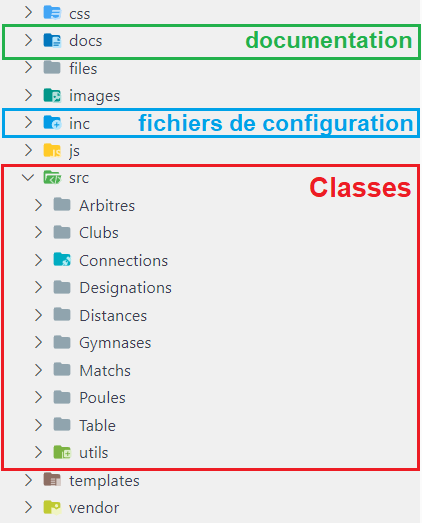
\includegraphics[width=0.5\linewidth]{architecture.png}
    \caption{Arborescence des dossiers du projet}
\end{figure}

\pagebreak

Pour effectuer cette séparation des fichiers sans compliquer l’utilisation des classes, j’ai adopté le concept de namespace et utilisé le gestionnaire de dépendances Composer pour ce projet.

\begin{commentaire}
    Composer est un gestionnaire de dépendances pour PHP. Il permet de réduire l’importation de fichiers en automatisant cette tâche.
\end{commentaire}

\vspace{2cm}

\faIcon{arrow-alt-circle-right} Je commencerai par expliquer les méthodes utilisées pour récupérer les données nécessaires à ce projet, puis j’exposerai les modifications apportées à l’interface graphique et enfin je parlerai en profondeur de l’algorithme d’automatisation des désignations. 


\section{Récupération des données}
\vspace{1cm}

Par manque d’accès à la base de données fédérale, la première étape consistait à récupérer les données nécessaires à la mise en place des outils.\\
Après une analyse complète des informations nécessaires au projet, j’en suis arrivé au modèle de données UML suivant :

\begin{figure}[!h]
    \centering
    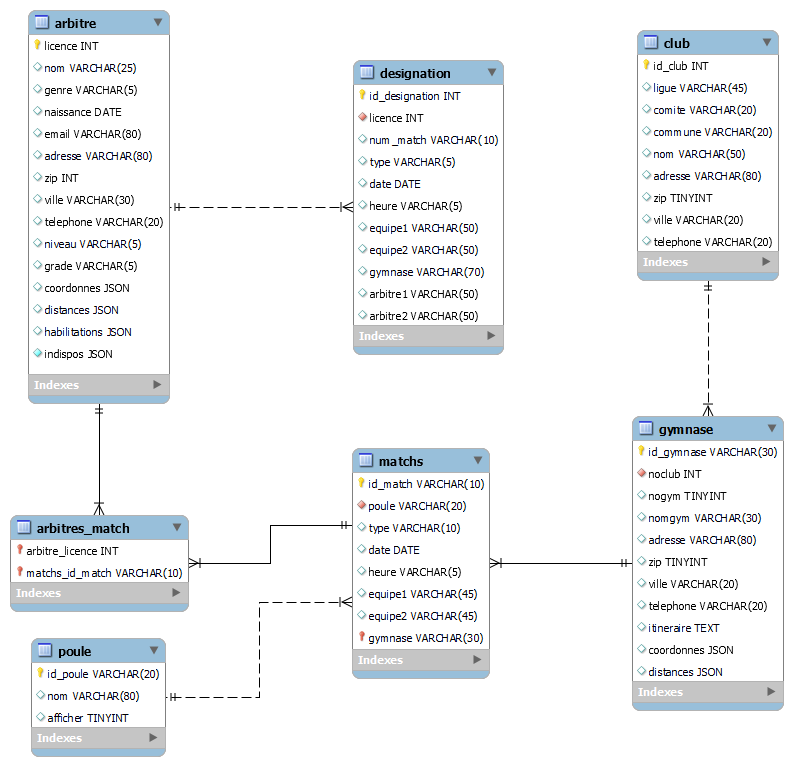
\includegraphics[width=\linewidth, height=15cm]{UML_DPP.png}
    \caption{Modèle de données UML effectué avec MySQL Workbench}
\end{figure}

\vspace{0.5cm}

Certaines données étaient disponibles au format csv (Excel), et d’autres demandaient à être récupérées sur l’intranet actuel de la fédération. Il m’a donc fallu extraire ces dernières via Web Scrapping pour ensuite les insérer dans ma base de données.
\subsection{Configuration}
\vspace{1cm}

Dans un premier temps, afin de faciliter la configuration de l’accès à la base de données lors de la mise en production, j’ai mis en place un fichier de configuration général \colored{globals.php}.\\
Ce fichier contenait un panel de variables de configuration différentes en fonction de l’environnement (développement ou production).
% bibliographie
\bibliography{mathbib}

\end{document}